\documentclass{extbook}[14pt]
\usepackage{multicol, enumerate, enumitem, hyperref, color, soul, setspace, parskip, fancyhdr, amssymb, amsthm, amsmath, latexsym, units, mathtools}
\everymath{\displaystyle}
\usepackage[headsep=0.5cm,headheight=0cm, left=1 in,right= 1 in,top= 1 in,bottom= 1 in]{geometry}
\usepackage{dashrule}  % Package to use the command below to create lines between items
\newcommand{\litem}[1]{\item #1

\rule{\textwidth}{0.4pt}}
\pagestyle{fancy}
\lhead{}
\chead{Answer Key for Progress Quiz 7 Version C}
\rhead{}
\lfoot{4173-5738}
\cfoot{}
\rfoot{Spring 2021}
\begin{document}
\textbf{This key should allow you to understand why you choose the option you did (beyond just getting a question right or wrong). \href{https://xronos.clas.ufl.edu/mac1105spring2020/courseDescriptionAndMisc/Exams/LearningFromResults}{More instructions on how to use this key can be found here}.}

\textbf{If you have a suggestion to make the keys better, \href{https://forms.gle/CZkbZmPbC9XALEE88}{please fill out the short survey here}.}

\textit{Note: This key is auto-generated and may contain issues and/or errors. The keys are reviewed after each exam to ensure grading is done accurately. If there are issues (like duplicate options), they are noted in the offline gradebook. The keys are a work-in-progress to give students as many resources to improve as possible.}

\rule{\textwidth}{0.4pt}

\begin{enumerate}\litem{
Construct the lowest-degree polynomial given the zeros below. Then, choose the intervals that contain the coefficients of the polynomial in the form $ax^3+bx^2+cx+d$.
\[ \frac{2}{3}, \frac{1}{2}, \text{ and } \frac{-7}{2} \]The solution is \( 12x^{3} +28 x^{2} -45 x + 14 \), which is option A.\begin{enumerate}[label=\Alph*.]
\item \( a \in [11, 24], b \in [26, 35], c \in [-50, -44], \text{ and } d \in [14, 21] \)

* $12x^{3} +28 x^{2} -45 x + 14$, which is the correct option.
\item \( a \in [11, 24], b \in [-29, -26], c \in [-50, -44], \text{ and } d \in [-16, -12] \)

$12x^{3} -28 x^{2} -45 x -14$, which corresponds to multiplying out $(3x + 2)(2x + 1)(2x -7)$.
\item \( a \in [11, 24], b \in [39, 45], c \in [3, 4], \text{ and } d \in [-16, -12] \)

$12x^{3} +44 x^{2} +3 x -14$, which corresponds to multiplying out $(3x + 2)(2x -1)(2x + 7)$.
\item \( a \in [11, 24], b \in [26, 35], c \in [-50, -44], \text{ and } d \in [-16, -12] \)

$12x^{3} +28 x^{2} -45 x -14$, which corresponds to multiplying everything correctly except the constant term.
\item \( a \in [11, 24], b \in [50, 60], c \in [53, 61], \text{ and } d \in [14, 21] \)

$12x^{3} +56 x^{2} +53 x + 14$, which corresponds to multiplying out $(3x + 2)(2x + 1)(2x + 7)$.
\end{enumerate}

\textbf{General Comment:} To construct the lowest-degree polynomial, you want to multiply out $(3x -2)(2x -1)(2x + 7)$
}
\litem{
Which of the following equations \textit{could} be of the graph presented below?

\begin{center}
    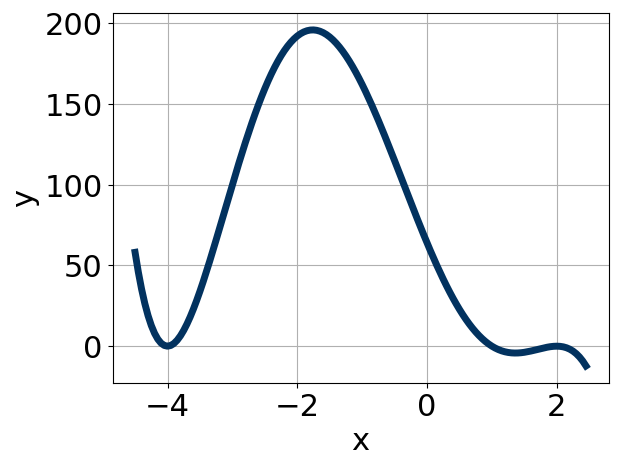
\includegraphics[width=0.5\textwidth]{../Figures/polyGraphToFunctionC.png}
\end{center}


The solution is \( -3x^{7} (x + 2)^{8} (x - 1)^{11} \), which is option D.\begin{enumerate}[label=\Alph*.]
\item \( 9x^{8} (x + 2)^{4} (x - 1)^{9} \)

The factor $x$ should have an odd power and the leading coefficient should be the opposite sign.
\item \( -2x^{5} (x + 2)^{8} (x - 1)^{4} \)

The factor $(x - 1)$ should have an odd power.
\item \( 13x^{11} (x + 2)^{10} (x - 1)^{7} \)

This corresponds to the leading coefficient being the opposite value than it should be.
\item \( -3x^{7} (x + 2)^{8} (x - 1)^{11} \)

* This is the correct option.
\item \( -9x^{5} (x + 2)^{9} (x - 1)^{8} \)

The factor $-2$ should have an even power and the factor $1$ should have an odd power.
\end{enumerate}

\textbf{General Comment:} General Comments: Draw the x-axis to determine which zeros are touching (and so have even multiplicity) or cross (and have odd multiplicity).
}
\litem{
Describe the zero behavior of the zero $x = 5$ of the polynomial below.
\[ f(x) = 8(x + 2)^{8}(x - 2)^{7}(x + 5)^{10}(x - 5)^{5} \]The solution is the graph below, which is option D.
\begin{center}
    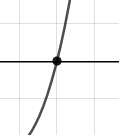
\includegraphics[width=0.3\textwidth]{../Figures/polyZeroBehaviorDC.png}
\end{center}\begin{enumerate}[label=\Alph*.]
\begin{multicols}{2}
\item 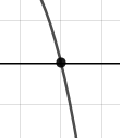
\includegraphics[width = 0.3\textwidth]{../Figures/polyZeroBehaviorAC.png}
\item 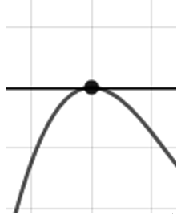
\includegraphics[width = 0.3\textwidth]{../Figures/polyZeroBehaviorBC.png}
\item 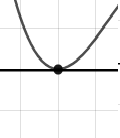
\includegraphics[width = 0.3\textwidth]{../Figures/polyZeroBehaviorCC.png}
\item 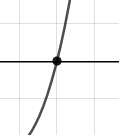
\includegraphics[width = 0.3\textwidth]{../Figures/polyZeroBehaviorDC.png}
\end{multicols}\item None of the above.\end{enumerate}
\textbf{General Comment:} You will need to sketch the entire graph, then zoom in on the zero the question asks about.
}
\litem{
Construct the lowest-degree polynomial given the zeros below. Then, choose the intervals that contain the coefficients of the polynomial in the form $x^3+bx^2+cx+d$.
\[ -4 - 3 i \text{ and } 2 \]The solution is \( x^{3} +6 x^{2} +9 x -50 \), which is option B.\begin{enumerate}[label=\Alph*.]
\item \( b \in [-1, 4], c \in [-0.36, 1.69], \text{ and } d \in [-6.6, -3.6] \)

$x^{3} + x^{2} +x -6$, which corresponds to multiplying out $(x + 3)(x -2)$.
\item \( b \in [5, 9], c \in [8.74, 10.07], \text{ and } d \in [-50.9, -49.8] \)

* $x^{3} +6 x^{2} +9 x -50$, which is the correct option.
\item \( b \in [-1, 4], c \in [1.92, 2.59], \text{ and } d \in [-10.8, -6.9] \)

$x^{3} + x^{2} +2 x -8$, which corresponds to multiplying out $(x + 4)(x -2)$.
\item \( b \in [-6, 0], c \in [8.74, 10.07], \text{ and } d \in [49.5, 51.7] \)

$x^{3} -6 x^{2} +9 x + 50$, which corresponds to multiplying out $(x-(-4 - 3 i))(x-(-4 + 3 i))(x + 2)$.
\item \( \text{None of the above.} \)

This corresponds to making an unanticipated error or not understanding how to use nonreal complex numbers to create the lowest-degree polynomial. If you chose this and are not sure what you did wrong, please contact the coordinator for help.
\end{enumerate}

\textbf{General Comment:} Remember that the conjugate of $a+bi$ is $a-bi$. Since these zeros always come in pairs, we need to multiply out $(x-(-4 - 3 i))(x-(-4 + 3 i))(x-(2))$.
}
\litem{
Construct the lowest-degree polynomial given the zeros below. Then, choose the intervals that contain the coefficients of the polynomial in the form $ax^3+bx^2+cx+d$.
\[ \frac{-7}{5}, \frac{1}{3}, \text{ and } \frac{1}{5} \]The solution is \( 75x^{3} +65 x^{2} -51 x + 7 \), which is option B.\begin{enumerate}[label=\Alph*.]
\item \( a \in [75, 82], b \in [-95, -92], c \in [-21, -16], \text{ and } d \in [1, 10] \)

$75x^{3} -95 x^{2} -19 x + 7$, which corresponds to multiplying out $(5x -7)(3x + 1)(5x -1)$.
\item \( a \in [75, 82], b \in [61, 66], c \in [-52, -46], \text{ and } d \in [1, 10] \)

* $75x^{3} +65 x^{2} -51 x + 7$, which is the correct option.
\item \( a \in [75, 82], b \in [61, 66], c \in [-52, -46], \text{ and } d \in [-14, -6] \)

$75x^{3} +65 x^{2} -51 x -7$, which corresponds to multiplying everything correctly except the constant term.
\item \( a \in [75, 82], b \in [-68, -60], c \in [-52, -46], \text{ and } d \in [-14, -6] \)

$75x^{3} -65 x^{2} -51 x -7$, which corresponds to multiplying out $(5x -7)(3x + 1)(5x + 1)$.
\item \( a \in [75, 82], b \in [-148, -139], c \in [57, 65], \text{ and } d \in [-14, -6] \)

$75x^{3} -145 x^{2} +61 x -7$, which corresponds to multiplying out $(5x -7)(3x -1)(5x -1)$.
\end{enumerate}

\textbf{General Comment:} To construct the lowest-degree polynomial, you want to multiply out $(5x + 7)(3x -1)(5x -1)$
}
\litem{
Describe the zero behavior of the zero $x = 3$ of the polynomial below.
\[ f(x) = -2(x + 3)^{5}(x - 3)^{10}(x - 6)^{4}(x + 6)^{5} \]The solution is the graph below, which is option B.
\begin{center}
    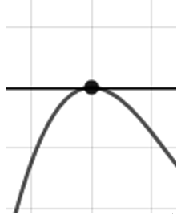
\includegraphics[width=0.3\textwidth]{../Figures/polyZeroBehaviorCopyBC.png}
\end{center}\begin{enumerate}[label=\Alph*.]
\begin{multicols}{2}
\item 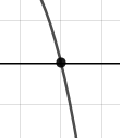
\includegraphics[width = 0.3\textwidth]{../Figures/polyZeroBehaviorCopyAC.png}
\item 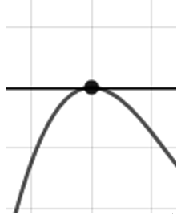
\includegraphics[width = 0.3\textwidth]{../Figures/polyZeroBehaviorCopyBC.png}
\item 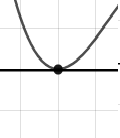
\includegraphics[width = 0.3\textwidth]{../Figures/polyZeroBehaviorCopyCC.png}
\item 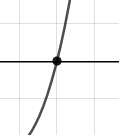
\includegraphics[width = 0.3\textwidth]{../Figures/polyZeroBehaviorCopyDC.png}
\end{multicols}\item None of the above.\end{enumerate}
\textbf{General Comment:} You will need to sketch the entire graph, then zoom in on the zero the question asks about.
}
\litem{
Describe the end behavior of the polynomial below.
\[ f(x) = 9(x - 7)^{3}(x + 7)^{8}(x + 8)^{3}(x - 8)^{4} \]The solution is the graph below, which is option C.
\begin{center}
    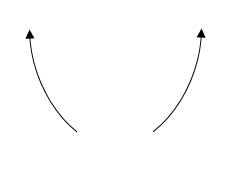
\includegraphics[width=0.3\textwidth]{../Figures/polyEndBehaviorCopyCC.png}
\end{center}\begin{enumerate}[label=\Alph*.]
\begin{multicols}{2}
\item 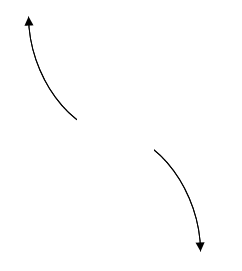
\includegraphics[width = 0.3\textwidth]{../Figures/polyEndBehaviorCopyAC.png}
\item 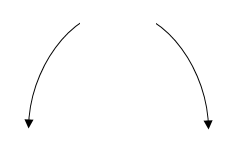
\includegraphics[width = 0.3\textwidth]{../Figures/polyEndBehaviorCopyBC.png}
\item 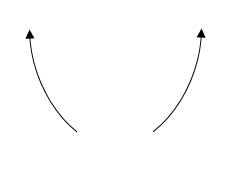
\includegraphics[width = 0.3\textwidth]{../Figures/polyEndBehaviorCopyCC.png}
\item 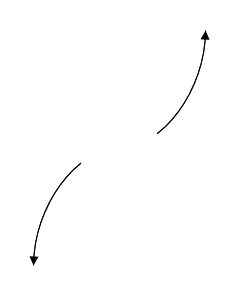
\includegraphics[width = 0.3\textwidth]{../Figures/polyEndBehaviorCopyDC.png}
\end{multicols}\item None of the above.\end{enumerate}
\textbf{General Comment:} Remember that end behavior is determined by the leading coefficient AND whether the \textbf{sum} of the multiplicities is positive or negative.
}
\litem{
Describe the end behavior of the polynomial below.
\[ f(x) = 4(x - 3)^{3}(x + 3)^{4}(x - 5)^{5}(x + 5)^{7} \]The solution is the graph below, which is option D.
\begin{center}
    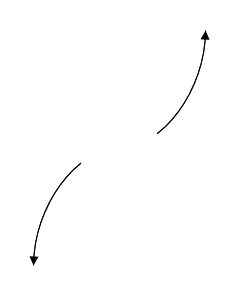
\includegraphics[width=0.3\textwidth]{../Figures/polyEndBehaviorDC.png}
\end{center}\begin{enumerate}[label=\Alph*.]
\begin{multicols}{2}
\item 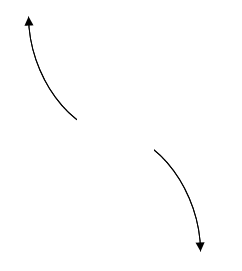
\includegraphics[width = 0.3\textwidth]{../Figures/polyEndBehaviorAC.png}
\item 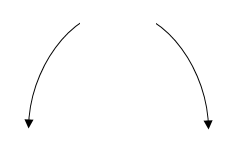
\includegraphics[width = 0.3\textwidth]{../Figures/polyEndBehaviorBC.png}
\item 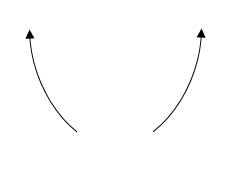
\includegraphics[width = 0.3\textwidth]{../Figures/polyEndBehaviorCC.png}
\item 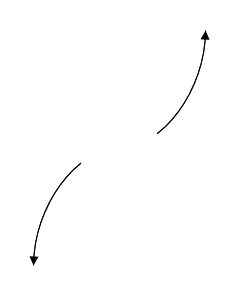
\includegraphics[width = 0.3\textwidth]{../Figures/polyEndBehaviorDC.png}
\end{multicols}\item None of the above.\end{enumerate}
\textbf{General Comment:} Remember that end behavior is determined by the leading coefficient AND whether the \textbf{sum} of the multiplicities is positive or negative.
}
\litem{
Which of the following equations \textit{could} be of the graph presented below?

\begin{center}
    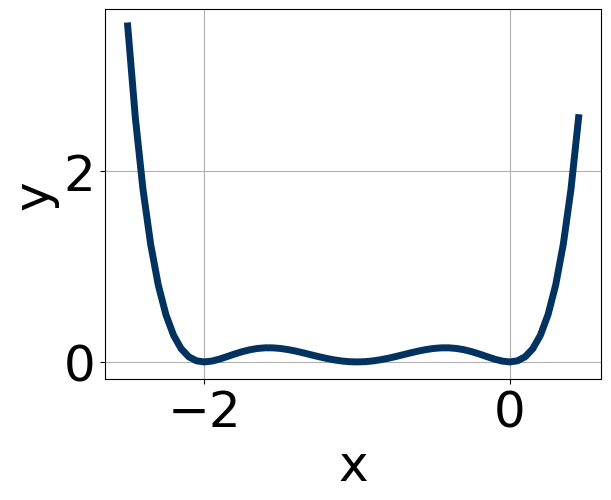
\includegraphics[width=0.5\textwidth]{../Figures/polyGraphToFunctionCopyC.png}
\end{center}


The solution is \( 5(x + 4)^{6} (x - 1)^{4} (x - 3)^{4} \), which is option C.\begin{enumerate}[label=\Alph*.]
\item \( -20(x + 4)^{10} (x - 1)^{4} (x - 3)^{10} \)

This corresponds to the leading coefficient being the opposite value than it should be.
\item \( 11(x + 4)^{4} (x - 1)^{5} (x - 3)^{11} \)

The factors $(x - 1)$ and $(x - 3)$ should both have even powers.
\item \( 5(x + 4)^{6} (x - 1)^{4} (x - 3)^{4} \)

* This is the correct option.
\item \( 14(x + 4)^{6} (x - 1)^{10} (x - 3)^{7} \)

The factor $(x - 3)$ should have an even power.
\item \( -8(x + 4)^{10} (x - 1)^{10} (x - 3)^{7} \)

The factor $(x - 3)$ should have an even power and the leading coefficient should be the opposite sign.
\end{enumerate}

\textbf{General Comment:} General Comments: Draw the x-axis to determine which zeros are touching (and so have even multiplicity) or cross (and have odd multiplicity).
}
\litem{
Construct the lowest-degree polynomial given the zeros below. Then, choose the intervals that contain the coefficients of the polynomial in the form $x^3+bx^2+cx+d$.
\[ -4 + 2 i \text{ and } 4 \]The solution is \( x^{3} +4 x^{2} -12 x -80 \), which is option A.\begin{enumerate}[label=\Alph*.]
\item \( b \in [2.8, 4.2], c \in [-12, -8], \text{ and } d \in [-83, -75] \)

* $x^{3} +4 x^{2} -12 x -80$, which is the correct option.
\item \( b \in [0.1, 2.1], c \in [0, 3], \text{ and } d \in [-19, -12] \)

$x^{3} + x^{2} -16$, which corresponds to multiplying out $(x + 4)(x -4)$.
\item \( b \in [-6.4, -3.6], c \in [-12, -8], \text{ and } d \in [79, 82] \)

$x^{3} -4 x^{2} -12 x + 80$, which corresponds to multiplying out $(x-(-4 + 2 i))(x-(-4 - 2 i))(x + 4)$.
\item \( b \in [0.1, 2.1], c \in [-10, -2], \text{ and } d \in [7, 12] \)

$x^{3} + x^{2} -6 x + 8$, which corresponds to multiplying out $(x -2)(x -4)$.
\item \( \text{None of the above.} \)

This corresponds to making an unanticipated error or not understanding how to use nonreal complex numbers to create the lowest-degree polynomial. If you chose this and are not sure what you did wrong, please contact the coordinator for help.
\end{enumerate}

\textbf{General Comment:} Remember that the conjugate of $a+bi$ is $a-bi$. Since these zeros always come in pairs, we need to multiply out $(x-(-4 + 2 i))(x-(-4 - 2 i))(x-(4))$.
}
\end{enumerate}

\end{document}